\chapter{Marco teórico: Inteligencia artificial y redes neuronales}

Las redes neuronales artificiales son un modelo de inteligencia artificial inspirado en el pensamiento humano, más específicamente, en cómo un conjunto de neuronas interconectadas comparten información. 	

Las redes neuronales artificiales son un conjunto de neuronas artificiales interconectadas que realizan cálculos y transmiten información para realizar una operación, imitando el comportamiento del cerebro.

Pero para entender este modelo, es necesario tener los fundamentos de inteligencia artificial y la clasificación de aprendizaje supervisado.

\section{Inteligencia artificial y aprendizaje supervisado}

La inteligencia artificial fue definida por primera vez por John McCarthy en 1955 como \textit{la ciencia e ingeniería de hacer máquinas inteligentes} \cite{ai_def_1}. Siguiendo a \cite{ai_def_1, ai_def_2, ai_def_3}, se propone la siguiente definición:

\begin{definition}
	
	La inteligencia artificial es la ciencia que utiliza modelos computacionales para crear sistemas capaces de realizar tareas que, si fueran hechas por humanos, requerirían inteligencia.
	
\end{definition}

Una de las ramas de la inteligencia artificial es el aprendizaje automático, el cual se centra en desarrollar sistemas con la capacidad de aprender en función de los datos \cite{ml_def_1}. Esto permite reconocer patrones y realizar predicciones a partir de grandes cantidades de datos \cite{GoogleCloud2025}.

Por lo que, con base en \cite{Oracle2025, IBM2025} podemos definir al aprendizaje automático de la siguiente manera:

\begin{definition}
	
	El aprendizaje automático es la disciplina que permite a las computadoras mejorar su desempeño en una tarea mediante la experiencia con datos, sin necesidad de instrucciones explícitas.
	
\end{definition}

Esta tecnología funciona trabajando a través del entrenamiento de algoritmos en conjuntos de datos para conseguir un resultado esperado. Es el proceso de optimizar el modelo para que pueda predecir la respuesta correcta. A mayor calidad en los datos de entrenamiento, mayor precisión se tendrá en el modelo \cite{GoogleCloud2025}.

El entrenamiento se refiere al proceso de enseñarle a un modelo de inteligencia artificial a realizar una o varias tareas mediante la exposición a grandes cantidades de datos \cite{training}. Este proceso facilita a los humanos el proceso de análisis de grandes volúmenes, especialmente en la era actual, donde se generan más datos que nunca en la historia \cite{oracle_ia}.

Dentro del aprendizaje automático se definen tres métodos en cómo una computadora puede aprender. Estos métodos son aprendizaje supervisado, no supervisado y por refuerzo.

\begin{itemize}
	
	\item El aprendizaje supervisado se caracteriza por el uso de conjuntos de datos etiquetados para entrenar algoritmos que clasifiquen datos o predigan resultados con precisión. Durante el proceso de entrenamiento, el modelo recibe entradas junto con las salidas correctas, lo que le permite al modelo ajustar sus parámetros hasta que sea capaz de realizar predicciones precisas sobre nuevos datos \cite{IBM2025}. 
	
	
	
	\item El aprendizaje no supervisado, a diferencia del supervisado, no necesita de un conjunto de datos etiquetados generados por el ser humano. Este tipo de aprendizaje puede descubrir patrones y estadísticas sin ninguna orientación o instrucción explícita \cite{GoogleCloud}. 
	
	
	
	\item El aprendizaje por refuerzo busca imitar la forma de aprendizaje humana de prueba y error. Este tipo de aprendizaje permite a las máquinas aprender a tomar decisiones y mejorar sus resultados con base en los errores cometidos \cite{AWS}.
	
	
	
\end{itemize}

IBM \cite{IBM2025} menciona algunos de los algoritmos más comunes de aprendizaje automático:

\begin{enumerate}
	
	\item \textbf{Redes neuronales:} Simulan el funcionamiento del cerebro humano, con un gran número de nodos de procesamiento conectados entre sí, llamados neuronas.
	
	\item \textbf{Regresión lineal:} Predice valores numéricos, con base en una relación lineal entre diferentes valores.
	
	\item \textbf{Regresión logística:} Realiza predicciones para variables de respuestas categóricas.
	
	\item \textbf{Agrupación en clústeres:} Identifican patrones en los datos y los agrupan en centroides.
	
	\item \textbf{Árboles de decisión:} Utilizan una secuencia ramificada de decisiones vinculadas que se representan con un diagrama de árbol.
	
	\item \textbf{Bosques aleatorios:} Combina los resultados de varios árboles de decisión y predice un valor o clasificación.
	
\end{enumerate}

Las redes neuronales presentan ventajas que pueden llegar a agilizar y optimizar recursos de las organizaciones que lo implementan \cite{Adobe2025}: mejora la productividad, reduce el error humano, mejora la disponibilidad de servicios, reduce tareas repetitivas, descubre patrones ocultos a simple vista, entre otros.

Para comprender cómo las redes neuronales logran estas capacidades, es necesario explorar primero los fundamentos que inspiraron el desarrollo. En particular, su diseño es una abstracción de las neuronas biológicas, cuya estructura y funcionamiento ofrecen una analogía al procesamiento de información.

\section{Neurona biológica}

Las neuronas son células especializadas del sistema nervioso cuyo objetivo es recibir, procesar y transmitir información por medio de señales químicas y eléctricas \cite{neurona_1, neurona_2}. 

Cada neurona se compone (principalmente) de tres elementos (como se muestra en la figura \ref{fig:neurona}): 

\begin{itemize}
	
	\item Las dendritas, que reciben señales provenientes de otras neuronas.
	
	\item El núcleo o cuerpo, que integra las señales provenientes de las dendritas y produce una nueva señal eléctrica.
	
	\item El axón, el cual conduce la señal producida por el cuerpo hacia otras neuronas haciendo sinapsis, es decir, transmite la señal de una célula a otra.
	
\end{itemize}

\begin{figure}[H]
	
	\centering
	
	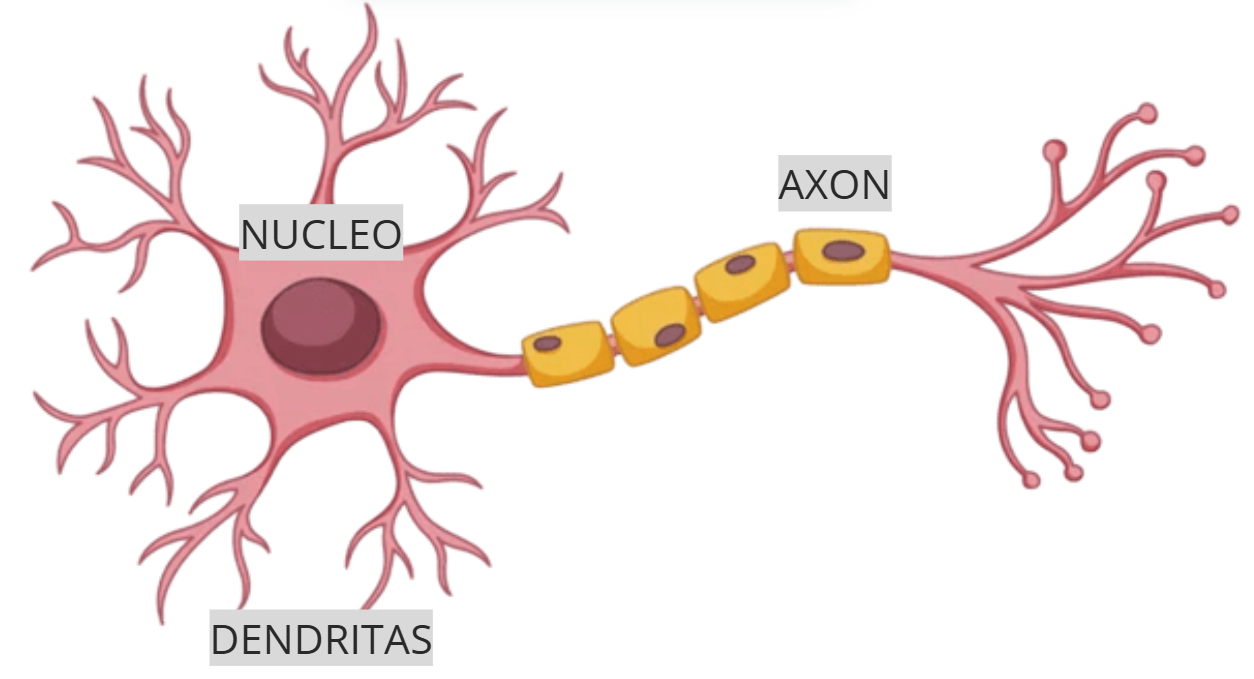
\includegraphics[width=0.6\linewidth]{img/neurona.png}
	
	\caption{Representación de una neurona \cite{img_neurona}. Se encuentran señaladas las dendritas, el núcleo y el axón, encargado de recibir, procesar y transmitir la información, respectivamente.}
	
	\label{fig:neurona}
	
\end{figure}

Las redes neuronales naturales son un sistema de neuronas que permite el procesamiento cerebral de la información; son altamente complejas, no lineales y con procesamiento en paralelo. 

\section{Neurona artificial} 

La neurona artificial se considera como una unidad de procesamiento de información \cite{neurona_1}. Sigue la misma estructura del modelo biológico con algunas consideraciones adicionales, como lo marcan \cite{neurona_1, neurona_artificial_1, neurona_artificial_2}:

\begin{itemize}
	
	\item Las dendritas equivalen al conjunto de datos de entrada. Sin embargo, no toda la información tiene la misma relevancia; para esto se le asigna a cada entrada un peso sináptico.
	
	
	
	\item El cuerpo se sustituye por dos funciones: (1) Una función de agregación que combina todos los datos de entrada (generalmente es una combinación lineal entre las entradas y los pesos sinápticos) y (2) una función de activación que determina si la neurona está activa y en qué grado. 
	
\end{itemize}

La cual se suele representar como en la figura \ref{fig:neurona_artificial}.

\begin{figure}[H]
	
	\centering
	
	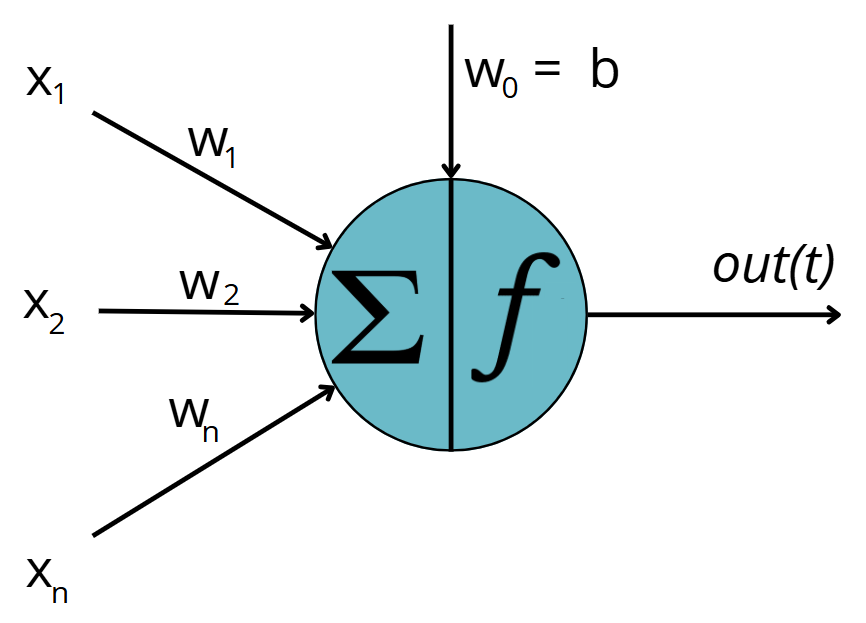
\includegraphics[width=0.6\linewidth]{img/neurona_artificial.png}
	
	\caption{Representación gráfica de una neurona artificial. Contiene las entradas ($x_1, x_2, \dots, x_n$), los pesos sinápticos ($w_1, w_2, \dots, w_n$), el sesgo ($w_0$ o $b$), la función de agregación ($\Sigma$), la función de activación ($f$) y la salida.}
	
	\label{fig:neurona_artificial}
	
\end{figure}

\begin{definition}
	
	Una neurona artificial es una función $f: \mathbb{R}^n \to \mathbb{R}$ dada por:
	
	\[
	f(x) = \phi (\omega (X, W, b))
	\]
	
	donde:
	
	\begin{itemize}
		
		\item $X = \{x_1, x_2, \dots, x_n\} \in \mathbb{R}$ es el conjunto de datos que recibe cada neurona.
		
		
		
		\item $W = \{ w_1, w_2, \dots, w_n \} \in \mathbb{R}$ es el conjunto de pesos sinápticos que indican la importancia de cada entrada.
		
		
		
		\item $b$ o $w_0 \in \mathbb{R}$ es un sesgo que desplaza la función de activación y controla el umbral de aceptación.
		
		
		
		\item $\omega(X,W,b)$ es una función de agregación $\omega: \mathbb{R}^n \to \mathbb{R}$ que combina las entradas. Usualmente se define como una combinación lineal:
		
		\[
		\omega(X,W,b) = \sum_{i = 1}^{n} w_i x_i + b
		\]
		
		
		
		\item $\phi(\omega(X,W,b))$ es la función de activación $\phi: \mathbb{R} \to \mathbb{R}$ que transforma $\omega(X,W,b)$ en una salida activada.
		
		
		
	\end{itemize}
	
	
	
\end{definition}

La función de activación es la que determina el valor de salida de cada neurona. Este valor, normalmente, se asigna entre un umbral para que limiten el comportamiento de la red neuronal \cite{funcion_activacion_1}.

\section{Redes neuronales}

Una neurona únicamente puede realizar una operación. Para aumentar la capacidad de entender patrones más complejos, es necesario añadir múltiples neuronas interconectadas, lo que se conoce como red neuronal artificial \cite{ann_1}. Esta puede definirse como un grafo dirigido \cite{ann_2}.

\begin{definition}
	
	Una red neuronal artificial es un grafo dirigido $G = (V, E)$ donde cada nodo $v \in V$ representa una neurona y cada arista $(u, v) \in E$ transporta la salida $y_u$ desde $u$ hasta $v$ ponderada por el peso $w_{uv}$. 
	
	
	
	Existe un conjunto de nodos de entrada $X \subseteq V$ que reciben los datos iniciales y un conjunto de nodos de salida $T \subseteq V$ cuya activación final representa la salida de la red.
	
\end{definition}

La red en su conjunto implementa una función parametrizada.

\[F_\theta: \mathbb{R}^n \to \mathbb{R}^m\] 

donde $n$ es el número de datos de entrada, $m$ el número de datos de salida y $\theta$ el conjunto de parámetros entrenables.

Por lo que podemos concluir con la definición de \cite{ann_3}, la cual dice que

\begin{definition}
	
	Una red neuronal es una función $F_\theta: \mathbb{R}^n \to \mathbb{R}^m$ donde $\theta = \{ w_{uv}, b_v : (u, v) \in E, v \in V \}$ es el conjunto de parámetros entrenables.
	
\end{definition}

\subsection{Aprendizaje en redes neuronales}

Dada una red neuronal artificial con los parámetros entrenables totalmente configurados, es capaz de realizar su clasificación o predicción de manera correcta. Sin embargo, resulta imposible configurar estos pesos manualmente, por lo que requiere de un ``entrenamiento'' que ayude a definir los pesos sinápticos. A continuación se define la función de pérdida, optimización y entrenamiento, elementos necesarios para obtener esa configuración específica.

\subsubsection{Función de pérdida}

La función de pérdida se usa para medir el rendimiento del modelo. Calcula la desviación que existe entre el valor predicho y el valor esperado. Esta función puede ser un escalar o un vector que permite aproximar la tasa de error para llegar a una solución óptima \cite{funcion_perdida_1}. 

\begin{definition}
	
	Sea $F_\theta$ una red neuronal artificial y $ \mathcal{D} = \{ (x^{(i)}, y^{(i)}) \}_{i = 1}^n $ un conjunto de datos de entrenamiento donde $x^{(i)}$ es la entrada y $y^{(i)}$ es la salida esperada; una función de pérdida es un mapeo. 
	
	\[
	\mathcal{L}: \mathbb{R}^m \times \mathbb{R}^m \to \mathbb{R}_{\geq 0}
	\]
	
	Tal que mide la discrepancia entre la predicción del modelo y la salida real:
	
	\[
	\mathcal{L} (F_\theta (x^{(i)}, y^{(i)}))
	\]
	
	
	
\end{definition}

Es importante que la función de pérdida sea diferenciable. El gradiente de la función de pérdida permite conocer la dirección hacia la cual debe moverse para disminuir la pérdida.

Las funciones de pérdida se pueden utilizar para regresión y para clasificación. La primera mide el error en valores continuos, usado para estimar valores contables como el precio, tamaño, tiempo. La segunda mide los errores en valores discretos, como la clasificación o la categoría.

Diferentes funciones de pérdida priorizan diferentes tipos de error; la elección de la función de pérdida dependerá de la tarea que se desea realizar. Además, la función de pérdida únicamente se limita a una muestra; para una población de muestras, se utiliza la función de costo, la cual se define a continuación \cite{funcion_perdida_1, funcion_perdida_2}:

\begin{definition}
	
	Sea $F_\theta$ una red neuronal artificial y $\mathcal{L}$ un conjunto de datos de entrenamiento; la función de costo es el promedio de las pérdidas:
	
	\[
	J(\theta) = \frac{1}{n} \sum_{i = 1}^{n} \mathcal{L}(F_\theta(x^{(i)}), y^{(i)})
	\]
	
\end{definition}

\subsubsection{Optimización}

El entrenamiento de una red consiste en ajustar los parámetros entrenables $\theta$ para minimizar la función de pérdida. La optimización resulta en resolver el problema de minimización dado por:

\[
\theta^* = \arg \min_{\theta} J(\theta)
\]

Esto se puede conseguir mediante diferentes técnicas, siendo el descenso del gradiente la más común. Este método actualiza los parámetros en la dirección opuesta al gradiente de la función de pérdida:

\[
\theta^{t + 1} = \theta^{(t)} - \eta  \nabla_\theta \mathcal{L}(\theta^{(t)})
\]

donde $\eta >0$ es la tasa de aprendizaje. Una tasa de aprendizaje alta puede divergir en la solución, mientras que una tasa baja puede tener una convergencia lenta \cite{ann_3}. 

\subsubsection{Entrenamiento}

Finalmente, el entrenamiento consiste en ajustar todos los parámetros $\theta = \{ W^{(l)}, b^{(l)}\}$ para minimizar la función de costos $J(\theta)$ en un conjunto de datos de entrenamiento. Este proceso se compone de las siguientes etapas:

\begin{enumerate}
	
	\item Se inicializan los parámetros, generalmente de forma aleatoria: $\theta_0 \sim \mathcal{D}_{init}$

	\item Se hace la propagación hacia adelante o \textit{forward pass}, es decir, para cada entrada $x^{(i)}$ se evalúa $\hat{y}^{(i)} = F_\theta(x^{(i)})$ 

	\item Se calcula la pérdida: $\mathcal{L}^{(i)} = \mathcal{L}(\hat{y}^{(i)}, y^{(i)})$
	
	\item Se calculan los gradientes propagando la información hacia atrás o \textit{backpropagation} utilizando la regla de la cadena.
	
	\[
	\nabla_\theta J(\theta) = \frac{1}{N} \sum_{i = 1}^{N} \nabla_\theta \mathcal{L} (F_ \theta(x^{(i)}, y ^{(i)}))
	\]

	Se actualizan los parámetros mediante la función de optimización: $\theta^{t + 1} = \theta^{(t)} - \eta  \nabla_\theta \mathcal{L}(\theta^{(t)})$

	\item Se repite este proceso sobre un \textit{dataset} hasta la convergencia de la solución o hasta alcanzar un criterio de parada \cite{ann_3}.
	
\end{enumerate}

En resumen, el entrenamiento de la red neuronal es un proceso iterativo de optimización que consiste en:

\begin{enumerate}
	
	\item Propagar los datos de entrada por la red.
	
	\item Comparar la salida con el valor real usando una función de pérdida.
	
	\item Propagar el error hacia atrás para obtener gradientes.
	
	\item Actualizar los parámetros con un algoritmo de optimización.
	
	\item Repetir hasta que el modelo aproxime adecuadamente la función deseada.
	
\end{enumerate}

Una vez comprendidas las redes neuronales, podemos retomar la definición de un autómata celular neuronal: una arquitectura que surge de la integración entre los autómatas celulares y las redes neuronales artificiales.

\clearpage